\documentclass[aspectratio=169]{beamer}
\usepackage{graphicx}
\setbeamertemplate{navigation symbols}{}
\begin{document}
\begin{frame}{FedAvg and first-round membership inference}
\scriptsize \textbf{Team 08} --- Assignment lead: Chetan Kodand Reddy Madadi\\
Team members: Bharat Govil, Naveen Jarpla, Vishnu Fnu
\begin{columns}[T]
\begin{column}{.54\textwidth}
\begin{itemize}
\setlength{\itemsep}{1pt}
\item 9,000 synthetic encounters; Assignment 1 generation pipeline reused.
\item 50/50 split: 3,600 SGD + 900 validation / 4,500 test.
\item 28 FedAvg settings $\times$ 3 seeds; 300-round cap.
\item L2 + validation scheduler; best validation checkpoint restored.
\item \textbf{Central synthetic validation is a simulation assumption.}
\item \textbf{72 loss-stable; 9 early stops; 3 capped.}
\item Baseline AUROC 0.657--0.707; validation-threshold BA 0.606--0.638.
\item $K=1$ test CE: 1.275 $\rightarrow$ 0.323; moderate predictive utility.
\end{itemize}
\end{column}
\begin{column}{.43\textwidth}
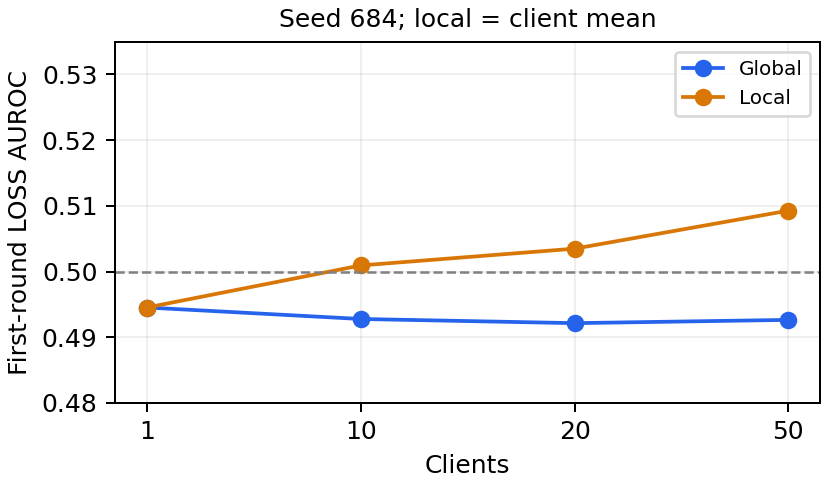
\includegraphics[width=\linewidth]{figures/attack_auc.png}
\scriptsize \textbf{Plot: seed 684 only.} Listed metrics are three-seed means. All 84 runs and 1,785 attacks audited.
First-round LOSS remains approximately chance; this is not a privacy guarantee.
\end{column}
\end{columns}
\medskip\scriptsize
Local nonmembers: all records outside that client's optimization partition.\quad
Oracle BA chooses its threshold retrospectively.\\
Secure aggregation hides individual updates; differential privacy limits membership leakage.
\end{frame}
\end{document}
